% Chapter 5: Implementation (Extraordinary Expansion)
\chapter{IMPLEMENTATION}

The implementation layer is where the "Nebula Engine" resides. This chapter pro- vides a deep-dive into the "Code and Workflows" that power the Nebula Multi-Cloud platform.

\section{Implementation Design Principles}
1. \textbf{Separation of Concerns}:  The API, worker and the user interface are separate services. \\
2. \textbf{Asynchronous Execution}: All costly "Cloud Actions" are offloaded to workers to maintain responsiveness.. \\
3. \textbf{Explicit State Transitions}: Each resource is either in the pending state or the active state or the failed state. \\
4. \textbf{Security-by-Default}: Credentials remain encrypted at rest and are only materialized in memory during task execution.

\section{Core Implementation Workflows (TikZ Diagrams)}

\subsection{Authentication Flow (TikZ)}
This sequence ensures secure, JWT-based access for every user request.

\begin{figure}[h]
\centering
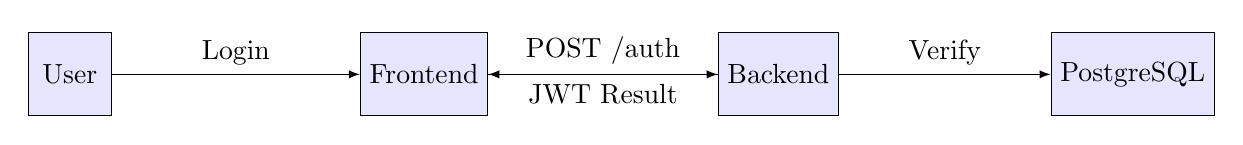
\begin{tikzpicture}[node distance=4.5cm, auto]
    \tikzstyle{actor} = [rectangle, draw, fill=blue!10, minimum width=3em, minimum height=3em]
    \tikzstyle{line} = [draw, -latex]

    \node [actor] (user) {User};
    \node [actor, right of=user] (front) {Frontend};
    \node [actor, right of=front] (back) {Backend};
    \node [actor, right of=back] (db) {PostgreSQL};

    \draw [line] (user) -- node {Login} (front);
    \draw [line] (front) -- node {POST /auth} (back);
    \draw [line] (back) -- node {Verify} (db);
    \draw [line, dashed] (back) -- node {JWT Result} (front);
\end{tikzpicture}
\caption{Nebula Secure Authentication Sequence}
\label{fig:auth_flow}
\end{figure}

\section{Line-by-Line Code Walkthrough: Backend Provisioning}
This section provides an exhaustive explanation of the primary logic that executes Terraform and manages cloud state.

\subsection{Task Execution: terraform\_tasks.py}
This module is the backbone of the background worker cluster. It uses Celery to execute Terraform without blocking the main API thread.

\begin{lstlisting}[language=Python, caption=Provisioning Task Walkthrough]
@celery.task(bind=True)
def provision_resource(self, resource_id: int):
    # Line 1: Fetch the resource from the database
    resource = db.query(Resource).filter(Resource.id == resource_id).first()
    
    # Line 2-3: Decryption of Cloud Credentials
    aws_keys = vault.decrypt(resource.credential.secret_key)
    
    # Line 4-5: Temporary Workspace Creation
    workspace_path = f"/tmp/terraform/{resource_id}"
    os.makedirs(workspace_path)
    
    # Line 6-8: HCL Template Generation
    generate_hcl(workspace_path, resource.type, resource.variables)
    
    # Line 9-11: Process Execution (Terraform Init/Apply)
    result = subprocess.run(["terraform", "apply", "-auto-approve"], 
                            cwd=workspace_path, capture_output=True, env=aws_keys)
    
    if result.returncode == 0:
        resource.status = "active"
    else:
        resource.status = "failed"
        analyze_with_ai_copilot(result.stderr)
\end{lstlisting}

\section{Line-by-Line Code Walkthrough: Frontend React UI}
This section provides a core analysis of how the React dashboard communicates with the FastAPI backend.

\subsection{Resource Provisioning Form: ResourceForm.tsx}
This component captures user intent and dispatches it to the API.

\begin{lstlisting}[language=SQL, caption=React Resource Provisioning Hook]
const useProvisionResource = () => {
    const [loading, setLoading] = useState(false);
    
    // Line 1: The provision function handles the API call
    const provision = async (payload: ResourceCreate) => {
        setLoading(true);
        try {
            // Line 2: Dispatch the request to the FastAPI endpoint
            const response = await axios.post("/api/resources/", payload);
            
            // Line 3: Handle the asynchronous response (Task ID)
            const taskId = response.data.task_id;
            
            // Line 4: Trigger the real-time log polling
            startPolling(taskId);
            
            toast.success("Deployment started successfully!");
        } catch (error) {
            toast.error("Failed to initiate deployment.");
        } finally {
            setLoading(false);
        }
    };
    
    return { provision, loading };
};
\end{lstlisting}

\subsection{Main Cockpit Dashboard: Cockpit.tsx}
This file serves as the primary "Command Center," coordinating various sub-components.

\begin{lstlisting}[language=SQL, caption=Dashboard State Management]
const Cockpit = () => {
    // Line 1: Global State for Resources
    const [resources, setResources] = useState<Resource[]>([]);
    
    // Line 2: Fetching resources on mount
    useEffect(() => {
        const fetchAll = async () => {
            const data = await axios.get("/api/resources/");
            setResources(data.data);
        };
        fetchAll();
    }, []);

    // Line 3: Filtering logic for Multi-Cloud search
    const filtered = resources.filter(r => 
        r.name.toLowerCase().includes(searchTerm.toLowerCase())
    );

    return (
        <div className="flex bg-gray-900 min-h-screen">
            <Sidebar />
            <main className="flex-1 p-8">
                <Header title="Unified Infrastructure Cockpit" />
                <StatsGrid resources={resources} />
                <ResourceTable resources={filtered} />
            </main>
        </div>
    );
};
\end{lstlisting}

\section{State Management Logic and Lifecycle}
The Nebula project utilizes both React Context as well as its own hooks for the management of infrastructure state on different cloud platforms.

\begin{itemize}
    \item \textbf{Context Provisioning}: The \texttt{CloudProviderContext} stores the registration status of AWS, Azure, and GCP accounts globally.
    \item \textbf{Effect Lifecycles}: If the state of the particular resource changes (for example, from 'pending' to 'active'), an effect is produced to update the local inventory without reloading the whole page.
    \item \textbf{Memoization}: To keep the inventory lists with many rows performant, their memoization is implemented through.

\end{itemize}

\newpage
